\chapter{Irodalom}
\pagestyle{headings}

Ebben a fejezetben a szakdolgozatom hátteréül szolgáló ismerető anyagot tekintem át. A fejezet két jól elkülönülő részből áll. Az első alfejezetben a pásztázó elektrokémiai mikroszkópia irodalmát mutatom be. A teljességre nem törekedve ismertetem kifejlesztésének főbb állomásait, a módszer működési elvét, fejlődését és felhasználási területeit. A fejezet második alfejezetében a pásztázó elektrokémiai mikroszkóp általam vizsgált új alkalmazási módjának példájául szolgáló Belouszov-Zsabotyinkszkij oszcilláló reakcióval foglalkozok. 

\section{Pásztázó elektrokémiai mikroszkópia}

\subsection{Története}

A PEKM a pásztázó mikroszkópos technikák egyik változata. Az első pásztázó mikroszkópos technikát, a pásztázó alagúthatás mikroszkópiát Binnig és Rohrer alkotta meg 1982-ben \cite{binnig1982surface}. Munkájukért mindössze négy évvel később, 1986-ban fizikai Nobel-díjat kaptak. A technika előnye, hogy rendkívül nagy felbontásra képes, akár atomokat is ,,láthatóvá tehetünk'', jóval meghaladva az optikai mikroszkópos technikák felbontását, melyek korlátozva vannak a használt fény hullámhosszúságára. A következő pásztázó technika az atomerő mikroszkóp (AFM, Atomic Force Microscope) viszonylag gyorsan jelent meg, szintén Binning és Rohrer munkájának köszönhetően \cite{binnig1986atomic, bennig1988atomic}. Azóta egy szerteágazó módszercsaláddá fejlődött az eredeti technika. Közös bennük, hogy egy -- általában szelektív -- mérőcsúcsot egy előre meghatározott ponthalmaz minden pontjára pozícionálunk, és lokális mérést végzünk. A mérés eredményét a helykoordinátákkal együtt tároljuk. A rögzített adatokból így képet készíthetünk, ábrázolva a mért mennyiséget a koordináták függvényében. A PEKM esetén a mérőcsúcs potenciometriás, vagy amperometriás. Az első hasonló mérést Engstrom végezte \cite{engstrom1986measurements}. Egy elektród diffúziós rétegében pásztázott egy másik, mikroméretű elektróddal. A mozgatáshoz egy mikromanipulátort használt. Ezzel mintegy három évvel előzte meg Allen J. Bardot és csoportját, akik kiforrott technikává fejlesztették a PEKM-et \cite{bard1989scanning}. A módszer eredetileg amperometriás detektálásra lett kifejlesztve. A potenciometriás változata azonban nem sokkal később jelent meg, Benjamin Horrocks és Nagy Géza munkájának köszönhetően \cite{horrocks1993scanning}.

\subsection{Működése}

A többi pásztázó technikához hasonlóan a PEKM alapja is a raszteres képalkotás. A képalkotás során a mérőcsúcsot mozgatjuk egy előre meghatározott program szerint. A program általában egy meander vonalat követ kétdimenziós pásztázás esetén, illetve egy vonal mentén pásztáz ide-oda egydimenziós pásztázás esetén. A mérési pontokon a mérőcsúcsot a program megállítja, és egy lokális mérést végez (\ref{fig:PEKM}. ábra). Amperometria esetén a mérőelektródot mozgatjuk, a segédelektród és a referenciaelektród egy meghatározott helyen áll, általában a cella szélén, távol a méréstől. Potenciometriás üzemmódban ionszelektív mikroelektródot használunk, és ennek potenciálját mérjük a referenciaelektródéhoz képest. Segítségével egy elektrokémiai, valós térbeli képet kaphatunk arról az ionféleségről, melyre a mikroelektród szelektív. Ezt a változatot használják többek között korróziós tanulmányokban a korrózió következtében kioldódott fémionok térképezésére \cite{bastos2010micropotentiometric, lamaka2008monitoring, karavai2010localized}. Munkám során potenciometriás PEKM-et használtam, a következő részben ezért kitérek a potenciometriás méréstechnikára.
\begin{figure}[!h]
\centering
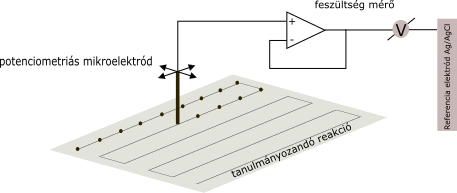
\includegraphics[width=0.8\textwidth]{img/PEKM.png}
\caption{Pásztázó elektrokémiai mikroszkóp működésének szemléltetése.}
\label{fig:PEKM}
\end{figure}


\subsection{Potenciometria} 

Az elektroanalitikai módszerek rendkívül szerteágazóak \cite{erdey1967, pfreisich1960, kissl1997}. A mérőcellában lévő mintába merülő elektródokat használunk, mely a vizsgálat típusától függően 2-4 lehet. Az elektródokat funkciójuk szerint különítjük el, lehet indikátorelektród, referenciaelektród (vonatkozási elektród) illetve segédelektród. Indikátor elektródként elsőfajú fémelektródokat, vagy 1-1 ionra szelektív elektródokat használhatunk, melyek lehetnek ionszelektív-, gáz-, redoxi- vagy enzimelektródok. Referenciaelektródnak másodfajú elektródokat alkalmazunk a méréseink során, amik egy fémből, a fém sójából és a só anionjának nagy koncentrációjú oldatából készül.

Az elektroanalitikai vizsgálatok közül a leggyakrabban alkalmazott módszer a potenciometria \cite{erdey1967}. A potenciometria során az elektrolitoldatba merített elektródok felületén kialakuló potenciál különbséget mérjük. Az elektrokémiai cella (jelen esetben galváncella) egy indikátor- és egy referenciaelektródból áll, e két félcella között mérjük a potenciálkülönbséget, miközben áram nem folyik át a cellán. Az elektródpotenciál és az elektród aktív komponens közötti összefüggést a Nernst-egyenlet adja meg:
\begin{equation}
E = E_\text{0} + \frac{RT}{zF} \ln a
\end{equation}
ahol $E$ a cellapotenciál, $E_\text{0}$ a rendszer standard potenciálja, $R$ a gázállandó, $T$ a termodinamikai hőmérséklet, $z$ az elektródfolyamat elektronszám-változása,az $F$ a Faraday-állandó, $a$ az elektródaktív komponens aktivitása.

Az aktivitás (a) és a koncentráció kapcsolatát az a=fc összefüggés adja meg, ahol f az aktivitási koefficiens. Híg oldatok esetén feltételezzük, hogy $f=1$, tehát $a=c$. A töményebb oldatok esetén, amikor $f\neq 1$, abban az esetben az aktivitási koefficiens állandó értéken tartásával és ily módon végzett kalibrációval kapunk analitikai információt. A gyakorlatban a fent említett Nernst-egyenletet koncentrációra felírva (c) és tizes alapú logaritmus formájában használjuk:
\begin{equation}
E= E_\text{0} + \frac{0.059}{z} \ln c
\end{equation}
Az elektródpotenciálból tehát az azt létrehozó elektródaktív komponens koncentrációja kiszámítható. Egy elektród felületén kialakuló feszültséget közvetlenül nem lehet mérni, ezért a vizsgálat során a keresendő komponens koncentrációja által generált potenciált mérjük az indikátorelektródon az állandó pontenciálú referenciaelektróddal szemben. Ezt az állandó potenciált a referenciaelektródon úgy tudjuk biztosítani, hogy a belső töltőoldatát állandó értéken tartjuk, ezt a referenciaelektród elválasztásával tudjuk elérni. A két elektród kapcsolódását sóhíd használatával valósítjuk meg. Azonban így egy új folyadék-folyadék határfelület jön létre, ami további potenciálkülönbséget eredményez. Ezt diffúziós potenciálnak nevezzük. A diffúziós potenciál a mérések során mindig fennáll, ugyanis nem tudjuk teljes mértékben megszűntetni. Ennek enyhítésére a sóhidat olyan elektrolittal készítik, melynek vizes oldatában az anionok és kationok mozgékonysága körülbelül megegyezik.

A kálium-,klorid- és a nitrátion mozgékonysága nagyjából megegyezik, ezért például használhatunk KCl és KNO$_3$ oldatot.
A fent említett oldatok esetén a diffúzió során a kation és az anion közel azonos sebességgel halad, így nem lesz töltésfeldúsulás. Fontos még, hogy a sóhídat képző oldat koncentrációja a vizsgálandó oldat és a referenciaelektród töltőoldatánál nagyobb legyen, ugyanis ilyenkor a sóhíd mindkét végén kifelé áramló diffúzió figyelhető meg. A sóhíd két végén fellépő diffúziónak az előjele ellentétes lesz, általában kiegyenlítik egymást.\\
%A potenciometriás méréseknél alkalmazott elektrokémiai cella potenciálját a %következőképpen kapjuk:
%\begin{equation}
%E= E_\text{i} - E_\text{v} + E_\text{d}
%\end{equation}
%ahol $E$ az elektrokémiai cella feszültsége, $E_\text{i}$ az indikátorelektródon a %meghatározandó komponens által generált feszültség, $E_\text{v}$ a viszonyító elektród %konstans potenciálja, $E_\text{d}$ a fent említett alacsony állandó értéken tartott %diffúziós potenciál.
A potenciometriás elektródok működésük alapján két csoportba sorolhatók:
\begin{itemize}
\item[•]ioncsere-egyensúlyon alapuló elektródok
\item[•]elektroncsere-egyensúlyon alapuló elektródok.
\end{itemize} 
Ebben a pontban csak a méréseim során használt elektródtípusokat mutatom be.
\begin{enumerate}
\item Redoxielektródok:\\
Működése elektroncsere-egyensúlyon alapul. Redoxi rendszerekben az inert fémek (pl.:Pt, Au) vagy grafitelektródok biztosítják az elektronoknak a vizsgálandó komponens redukált formájából az oxidált formába való folyamatos átmenetével járó egyensúlyt. A mért potenciál értéket a Nernst-Peters-egyenlet értelmében, a redoxirendszer oxidált és redukált formáinak koncentráció hányadosa adja meg:
\begin{equation}
E= E_\text{0} + \frac{0,059}{z} * \frac{[ox.]}{[red.]}
\end{equation}
A munkám során a redoxielektród platina és szénszálelektród formájában került alkalmazásra.
\item Elsőfajú fémelektródok:\\
Azon fémek alkalmasak elsőfajú elektród alapanyagának, melyeknél a  fém felületén kialakuló feszültség a saját ionjait tartalmazó oldatba merülve Nernst-i viselkedést mutat, az elektród potenciálját csak az oldatban lévő ionjaik aktivitása határozza meg. Elsőfajú elektróddal fémionkoncentráció és fémionaktivitás mérhető.Az elektród nem készíthető olyan fémekből, amik oldatban passziválódnak (vas, kobalt, nikkel és alumínium) viszont ezüstből, ólomból, kadmiumból, higanyból, ónból, bizmutból, cinkből és talliumből gond nélkül készíthető elsőfajú elektród. A legelterjedtebb az ezüst- és a higanyelektród.
\item Másodfajú elektród: \cite{pfreisich1960}\\
A másodfajú elektródokat többnyire referencia (viszonyító) elektródként alkalmazzák. A gyarlatban használt másodfajú elektródok például az Ag/AgCl és Hg/Hg$_2$Cl$_2$, amelyek egy fémból, a fém sójából, valamit a nehezen oldható só anionjának nagy koncentrációjú oldatából áll. Ezüst-klorid elektród esetén az elektród potenciálját az oldatban lévő ezüst-ionok aktivitása határozza meg.\\
\begin{equation}
E = E_0 + 0.059 \times \lg [Ag^+]
\end{equation}
mivel az oldat AgCl-re nézve telített az oldat ezüst-ion koncentrációjának és klorid-ion koncentrációjának szorzata állandó és egyenlő az oldhatósági szorzattal.\\
\begin{equation}
K = [Ag^+] \times [Cl^-]
\end{equation}
Az oldat klorid-ion koncentrációját részben az oldott AgCl, részben az oldat KCl határozza meg, de az ezüst-klorid rendkívül kis oldhatósága miatt az oldat klorid-ion koncentrációját a KCl-ból származó klorid-ion koncentrációja fogja meghatározni az AgCl-ból származó klorid-ion koncentrációt elhanyagolható.\\
\begin{equation}
E = E_\text{0} + 0,059 \lg \frac{K}{Cl^-} = E_\text{0} + 0,059 \lg K - 0,059 \lg [Cl^-]
\end{equation}
\begin{equation}
E = E_\text{0} - 0,059 [Cl^-]
\end{equation}
A fenti egyenletekből következik, hogy az ezüst-klorid elektród potenciálját az oldat anion koncentrációjának változása fogja meghatározni, ugyanis az oldatban lévő anion koncentráció határozza meg az ezüst-ion koncentriációt.
\end{enumerate}
    

\section{A Belouszov-Zsabotyinszkij oszcilláló reakció}
Dolgozatom elsősorban a PEKM technika új alkalmazási területével foglalkozik, a Belouszov-Zsabotyinszkij reakciót pedig csak modellrendszerként használtam munkám során. Témavezetőmmel olyan rendszert kerestünk, melyben jelentős ionaktivitás grádiens léphet fel homogén folyadékfázisú rendszerben. Megfelelő példának tűnt a BZ-reakció, melynek keveretlen lefolyása esetén térbeli mintázatok alakulnak ki. A térbeli mintázatok mentén változik többek között a bromid-ion aktivitás és a redox-potenciál, két olyan paraméter, melyek kiválóan mérhetők potenciometriás PEKM technikával. Ezek közül a redox-potenciál térképezését választottam. A továbbiakban áttekintem az oszcilláló jelenségeket, bemutatom a BZ-reakció főbb irodalmát, különös tekintettel a vizsgálati módszerekre.

\subsection{Oszcilláló jelenségek}
Oszcilláló jelenségeket a hétköznapi életben is megfigyelhetünk, ha szabályos időközönként ugyanaz az esemény megismétlődik, akkor időben periodikus eseményről, azaz oszcillációról beszélünk. Ezek az események számos tudományban megfigyelhetőek. Legegyszerűbb példa lehet a nap-éj periodikus váltakozása, megemlíthetjük még az évszakok váltakozását, mint csillagászati példa.

Az emberi szervezetben is megfigyelhetőek oszcilláló viselkedések, például a szív jobb pitvarának falában lévő szinuszcsomókban elhelyezkedő sejtek által küldött periodikus jelek hatására  szívünk átlagosan 72-szer húzódik össze percenként. Matematikai oszcilláló jelenség a szinusz és koszinusz periodikus függvények. Az állatvilágban (biológia) is megfigyelhetünk ilyen jelenségeket a zebrák és oroszlánok populációjának változása, amennyiben sok zebra van és kevés oroszlán az oroszlánok száma növekedni fog, míg a zebráké csökken és ez a populációs arány változik periodikusan. Fizika tudomány területén megemlíthetjük a harmonikus rezgőmozgásokat, mechanikai ingát,  az elektronikai “flip-flop” jelenséget. Ezekre rávilágítva belátjuk, hogy az univerzum számos oszcilláló jelenséget produkál, sőt Lawrence Mead és Harry Ringermacher elmélete \cite{ringermacher2017strong}  szerint maga az univerzum is oszcillál, tágulása a múltban lelassult, majd újra felgyorsult és ez a folyamat felelős az univerzum egyes folyamataiért. Ez a jelenség feltételezéseik szerint már 7 periódust oszcillált az évmilliárdok során.

\subsection{Kémiai oszcilláció}
A kémiai oszcilláló rendszerek ismerete a XVII. század végére vezethető vissza.  A kémiai jelenségeknél megkülönböztetünk homogén és heterogén rendszereket. A homogén és heterogén oszcilláló rendszereket Alan Turing matematikai úton leírta.\cite{turing1952chemical} A heterogén rendszerek felfedezésével kezdődött a kémiai reakciók kronológiája, mikor Robert Boyle \cite{harvey1957history} felfedezte az elemek égetésekor történő tömegnövekedés vizsgálata során a foszfor oxidációjakor fellépő halvány luminesszencia felvillanásokat, amik periodicitást mutatattak. Őt követte  Fechner 1828-ban felfedezett áramoszcillációja \cite{fechner1828schweigg}, amikor gyengén megsavanyított ezüst-nitrát oldatba merített ezüst- és vaselektródok között áram- és feszültségoszcillációt észlelt. 1896-ban a német kémikus Liesegang periodikus csapadékképződést figyelt meg \cite{liesegang1896ueber}, híg kálium-bikromátból és zselatinból készült gél felszínére tömény ezüst-nitrátot cseppentett, ahol néhány óra elteltével a gél és az ezüst-nitrát határfelületénél csapadéksáv keletkezik, az idő előrehaladtával kialakulnak az úgynevezett Liesegang-gyűrűk. 1899-ben Ostwald \cite{ostwald1899jacobus} periodikus H$_2$ fejlődést tapasztalt króm sósavban való oldásakor.

1943-ban Frank-Kamenyeckij termokémiai oszcillációkat tanulmányozott \cite{frank1943nikov}, ezek legismertebb példája a hideglángok jelensége, amely során egy alkán alacsony hőmérsékleten történő tökéletlen égésekor szabályos időközönként megjelenő halványkék lángot tapasztalt a reakciótérben.
Heterogén oszcilláló jelenség jól megfigyelhető a „higanyszív” nevezetű reakció esetében is, amely során kálium-bromátos híg kénsavoldatban lévő higany csepphez egy vasszöget érintve a higany pulzáló mozgást végez. Ezt a jelenséget a higany- és a vas felületén lejátszódó bonyolult elektrokémiai jelenséggel magyarázhatjuk, ahol az oldatban lévő higany pozitív a vas negatív töltésű. A tű érintésére a töltés közömbösítődik, ezért a higanycsepp összerándul, majd ezt az összerándulást periodikusan folytatja.

\subsection{A bromát-oszcillátor} \label{bromatoszcillator}
Az oszcilláló reakciók lényege a negatív visszacsatolás, ami megakadályozza egy közti termék koncentrációjának megszaladását. Az oszcilláció kialakulásának feltételei:
\begin{enumerate}
\item a termodinamikai egyensúlytól távoli rendszer
\item instabilitást előidéző kémiai reakciók a mechanizmusban:
 \begin{itemize}
\item pozitív visszacsatolás (autokatalízis)
\item negatív visszacsatolás (inhibíció)
\end{itemize}
\end{enumerate}
Kémia oszcillálóról akkor beszélünk, ha a reakcióban résztvevő komponensek koncentrációja nem monoton, hanem periodikusan változik. Koncentráció oszcilláció megjelenhet az idő illetve a térskálán. Amennyiben az időskálán jelenik meg a koncentráció oszcilláció, akkor az oszcilláló komponens koncentrációjával arányos jel nyomon követhető például elektródpotenciál mérésével.\cite{miklososzcillalo}
Az oszcilláló jelek lehetnek szabályosak (periodikus) illetve szabálytalanok (aperiodikus). Szabálytalan jeleket kémiai káosznak nevezik. A koncentráció oszcilláció előbbiekben említett módon a térkoordináták mentén is kialakulhatnak, ebben az esetben kémiai mintázatok alakulnak ki az oszcilláció kinetika és diffúzió következtében.
%A BZ-reakció a mintázatképződés modellje. A mintázatképződés biológiai szempontból rendkívül fontos, ugyanis az élőlények genetikai és fejlődési mintázata meghatározza az anatómiai részek egymáshoz viszonyított helyzetét, az élőlények összes alaki tulajdonságait. Mára bebizonyosodott, hogy a biológiai rendszerekben is hasonló mintázatok alakulnak ki, mint az általam tanulmányozott BZ-reakcióban, gondolok itt elsősorban a Xenopus embrióban kialakuló mintázatokra. \cite{chang2013mitotic}
\begin{figure}[!h]
\def\s{0.17}
\centering
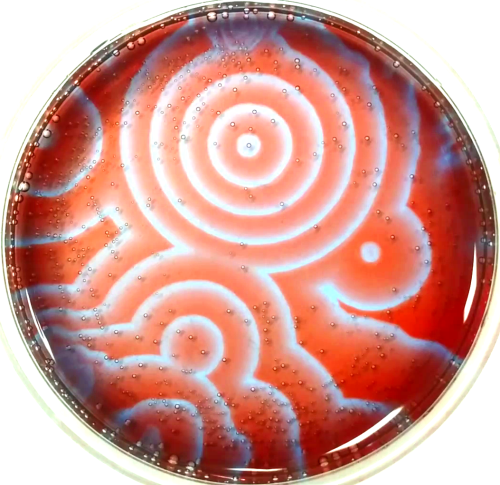
\includegraphics[width=\s\textwidth]{img/sequence/0001.png}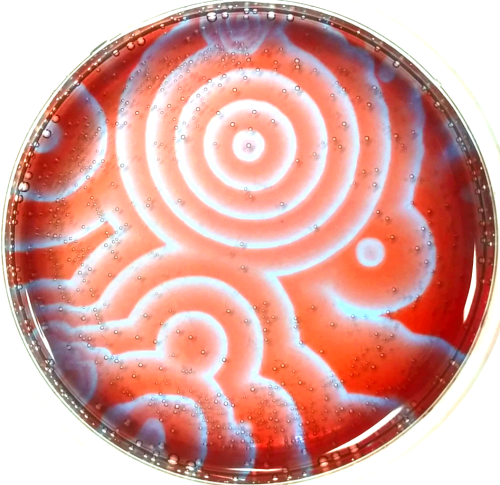
\includegraphics[width=\s\textwidth]{img/sequence/0111.png}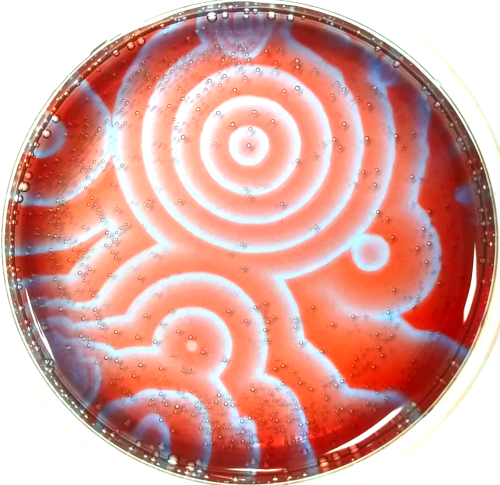
\includegraphics[width=\s\textwidth]{img/sequence/0221.png}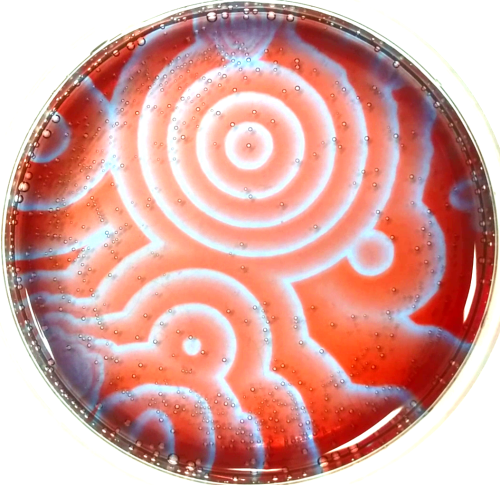
\includegraphics[width=\s\textwidth]{img/sequence/0331.png}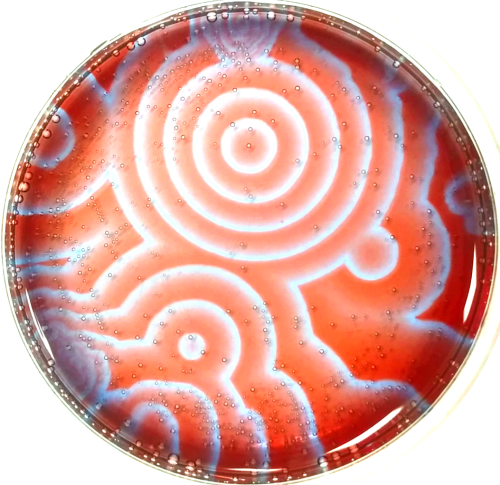
\includegraphics[width=\s\textwidth]{img/sequence/0441.png}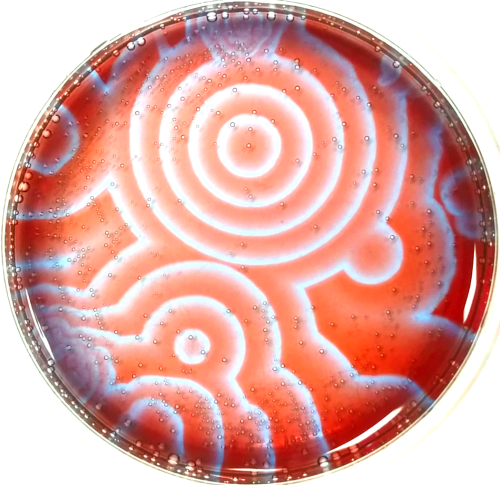
\includegraphics[width=\s\textwidth]{img/sequence/0551.png}
\caption{Kvázi kétdimenziós BZ-reakció Petri-csészében. A képeket 4 másodperces időközönként ragadtam ki a reakcióról készített videóból.}
\label{fig:bzsequence}
\end{figure}

A kémiai mintázatok dinamikus vagy stacionárius formában jelenhetnek meg. Dinamikus formai megjelenés a mozgó kémiai hullámok, amelyek az idő előrehaladtával növekvő sugarú koncentrikus köröket képeznek (\ref{fig:bzsequence}. ábra). Ezeket megzavarva jobbra- vagy balra forgó spirálok alakulhatnak ki.
Stacionárius térbeni szerkezetek esetében állóhullámok jelenhetnek meg, ilyen például a Turing struktúra, ami labirintus formájú sávok, vagy szabályos pontok térbeli mintázata.

Ugyan az első homogén fázisú oszcillálló jelenséget -- jodátion katalizált hidrogén-peroxid bomlásakor megfigyelhető oszcillációt -- Bray fedezte fel 1921-ben \cite{bray1921periodic}, a leghíresebbet Belouszov írta le 1955-ben \cite{belousov1959collection}. Felfedezte, hogy citromsav kénsavas közegben és Ce(IV)/Ce(III) ionokkal katalizált bromátos oxidációja során az oldat színe a katalizátor oxidált (sárga szín) és redukált állapotára (színtelen) jellemző színek között oszcillál.

A reakciót Zsabotyinszkij továbbfejlesztette és adta meg a Belouszov reakció vázmechanizmusát.\cite{zhabotinsky1964periodical} Az eredeti reakcióban Belouszov által használt citromsavat, mint szerves szubsztrátot malonsavval helyettesítette, a Ce(IV) helyett ferroin indikátort vagy Mn(II)-t alkalmazott katalizátorként, így a reakció általános összetétele: Bromát-Szubsztrát-Katalizátor-Sav.\cite{miklososzcillalo}
Minden olyan reakciót, ahol valamilyen szerves szubsztrátumot oxidálunk savas bromáttal átmeneti-fémionok jelenlétében Belouszov-Zsabotyinszkij reakciónak nevezünk. Erre a reakcióra Richard J. Field, Kőrös Endre, Richard M. Noyes kidolgoztak egy modellt \cite{noyes1972oscillations}, amit a nevük után Field-Kőrös-Noyes (FKN) modellnek neveznek. A mechanizmus során a rendszer két kinetikai (A és B kinetikai állapot) állapot között oszcillál, amit három részfolyamatra oszthatunk. A reakció kinetikai állapotát a bromid-ion koncentráció határozza meg.
Az első állapotban (A állapot) során a rendszer bromid-iont fogyaszt, így annak koncentrációja folyamatosan csökken. Amikor a bromid-ion koncentráció elér egy kritikus minimum értéket, a reakció a második kinetikai állapotba kerül (B állapot). A második kinetikai állapot során a redukált katalizátor (ferroin-indikátor) oxidálódik. A B állapot fontos jellemzője, hogy brómossav képződik autokatalitikus módon. Ahhoz, hogy a reakció oszcillálhasson, el kell jutnunk B-ből A-ba. Ez az oxidált katalizátor redukciójával valósul meg. Ennek során bromid-iont termel a rendszer (R10) így az első kinetikai állapotba jutunk (A állapot), ahol a ciklus újra kezdetét veszi. A reakció során a katalizátor (ferroin) oxidált és redukált aránya oszcillál, ezt az analitikai paramétert vizsgáltam a munkám folyamán. A nettó reakciók:\\
\ce {BrO3^- + Br- + CH2(COOH)2 + 3 H+ -> 3 BrCH(COOH)2 + 3 H2O} (A)\\
\ce {BrO3^- + Fe^2+ + CH2(COOH)2 + 5 H+ -> BrCH(COOH)2 + 4 Fe^3+ + 3 H2O} (B)\\
\ce {4 Fe^3+ + BrCH(COOH)2 + 2 H2O -> Br- + 4 Fe^2+ + HCOOH + 2 CO2 + 5 H+} (R10)\\
\ce {CH2(COOH)2 + 6 Fe^3+ + 2 H2O -> 6 Fe^2+ + HCOOH + 2 CO2 + 6 H+} (R9)\\
\ce {3 BrO3^- + 5 CH2(COOH)2 + 3 H+ -> 3 BrCH(COOH)2 + 2 HCOOH + 4 CO2 + 5 H2O} (C)

Meg szeretném említeni, hogy a homogén fázisú oszcilláló reakciók tanulmányozásának erős magyar vonatkozása van. Már igen korán tanulmányozta Kőrös Endre a reakciót, a korábban is hivatkozott közleményekben \cite{field1974oscillations, noyes1972oscillations} szerzőtársaival felállított egy modellt, mely kielégítő magyarázatot adott a reakcióra. Megemlítendő még Orbán Miklós akadémikus pH--oszcillátorokkal kapcsolatos munkája \cite{orban2015ph}, Szalai István mintázatképződéssel foglalkozó munkája \cite{molnar2015pattern}, Noszticzius Zoltán BZ-reakcióval kapcsolatos munkája \cite{noszticzius1987sustained} illetve Bánsági Tamás tomográfiás vizsgálatai \cite{bansagi2011tomography}.

\subsection{A BZ-reakció a biológiai mintázatképződés modellje}

A híres matematikus és polihisztor, Alan Turing vetette fel, hogy a biológiai mintázatok kialakulása magyarázható pusztán reakció--diffúzió rendszerekkel \cite{turing1952chemical}. \emph{,,The chemical basis of morphogenesis,,} című művében, pusztán matematikai alapon megjósolta az oszcilláló reakciók létezését, mielőtt azokról bármilyen kísérletes eredmény született volna. Hogy ez valóban így van-e, sokáig nem lehetett tudni. Kőrös Endre 1972-es publikációjában írta, hogy \emph{,,Csak a jövő a megmondhatója, hogy a BZ-reakció több-e mint laboratóriumi érdekesség,,} \cite{field1972oscillations}. Ma már biztosan tudjuk, hogy ezen reakciók nagy jelentőségűek a biológiai mintázatképződés szempontjából is, és a biológiai mintázatképződés szinte teljesen megmagyarázható reakció--diffúzió rendszerekkel \cite{kondo2010reaction}. A mintázatképződés az a folyamat, mely során az a hihetetlen, több nagyságrenden átívelő szerveződés kialakul, amit például egy emberi szervezet mutat, a viszonylag egyszerű zigótából. Ez a fejlődésbiogia központi kérdése. A biológiai rendszerekben a BZ-reakcióhoz hasonló oszcillátorok működnek. Ilyen például az embriogenezis során kulcsfontosságú Cdk1--APC/C oszcillátor \cite{yang2013cdk1}. A jól jellemzett \emph{Xenopus} zigótában is megfigyeltek hasonló oszcillációt, mely valószínűleg az első néhány leánysejtet eredményező osztódás térbeli koordinációját irányítja \cite{chang2013mitotic}. Egy látványos érdekességet szeretnék bemutatni a \ref{fig:csiga}. ábrán. Jól látható a csigaházon az elágazó ék--mintázat. A kialakulását könnyen meg lehet érteni, ha fontolóra vesszük, milyen mintázatot kapnánk, ha a BZ-reakciót tér--idő diagramon ábrázolnánk. A táguló koncentrikus körbe rendeződő kémiai hullámok egy ilyen diagramon egymásra rétegzett ékeknek látszanának, pontosan amit a csigaházon látunk. A spirál alakban növekedő csigaház ilyen tekintetben olyan, mint egy tér--idő diagram. A BZ-reakció tehát nem csak érdekesség, hanem a biológiai mintázatképződés megértéséhez is fontos lehet.

\begin{figure}[!h]
\centering
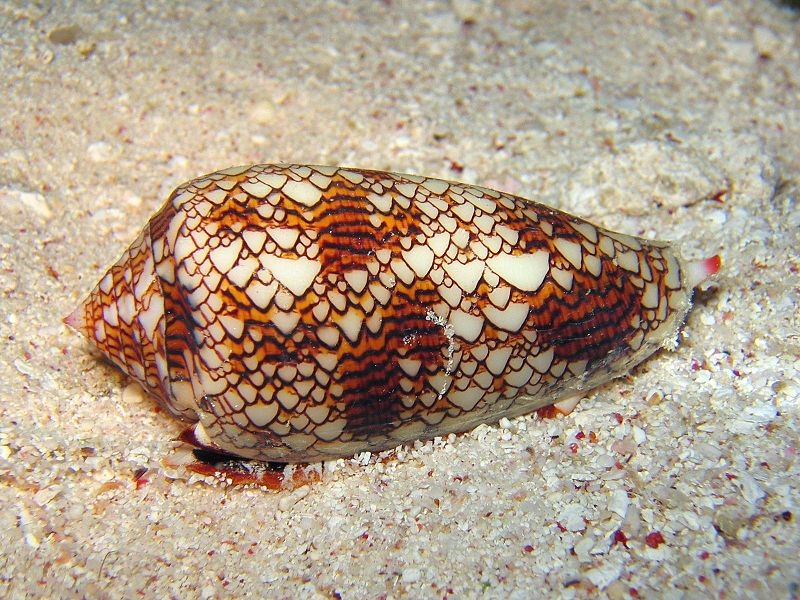
\includegraphics[width=0.6\textwidth]{img/conus.jpg}
\caption{\emph{Conus textile} csiga háza. A kialakuló mintázat hasonló egy tér--idő síkon ábrázolt kvázi--kétdimenziós BZ-reakcióhoz.}
\label{fig:csiga}
\end{figure}
